\section{第二类算子方程}
\label{sec:opeq-second-kind}

另一类方程中，未知函数同时出现在算子里面和外面：$u$等于已知的源项加上$u$自身的一个积分平均。写成矩阵，就是$(\bm I-\lambda\bm A)\bm x=\bm b$。多出来的这个恒等项看起来不起眼，却改变了方程的全部性质。本节先在贯穿例子上比较两类方程，再分两步研究可解性：参数较小时直接构造逆，一般参数下建立Fredholm择一。

\paragraph{方程与恒等项}
设$H$为Hilbert空间，$K:H\to H$为紧算子。与第一类方程不同，这里输入和输出必须在同一个空间中，$u$与$Ku$才能相减。

\begin{definition}[第二类算子方程]
\label{def:opeq-second-kind}
给定紧算子$K:H\to H$、参数$\lambda\in\mathbb F$与$f\in H$，求$u\in H$使
\begin{equation}
  (I-\lambda K)u=f,
  \label{eq:opeq-second-kind}
\end{equation}
称为\term{第二类算子方程}（operator equation of the second kind）。若$K$是核为$k$的积分算子，方程写成
\begin{equation}
  u(x)-\lambda\int k(x,z)u(z)\,\mathrm d\mu(z)=f(x),
  \label{eq:opeq-second-kind-integral}
\end{equation}
也称为第二类积分方程。
\end{definition}

回到秩二算子$T$，它在三类方向上分别乘以$1$、$\frac13$、$0$。把$u=\alpha+\beta x+h$与$f=a+bx+r$按同样的方式分解，$h,r$都与$1,x$正交，逐方向比较系数：
\begin{equation}
  (1-\lambda)\alpha=a,\qquad
  \Bigl(1-\frac\lambda3\Bigr)\beta=b,\qquad
  h=r.
  \label{eq:opeq-rank-two-second}
\end{equation}

只要$\lambda\neq1,3$，每个$f$都给出唯一解。例如$\lambda=\frac12$时，三个方向的结果是
\[
  \alpha=2a,\qquad \beta=\frac65b,\qquad h=r.
\]
第一类方程把正交补方向压成零，信息丢失；这里$I-\lambda T$在这些方向上恰好是恒等作用，信息完好。图~\ref{fig:opeq-equation-types}把这一差别画成各方向上的乘子：蓝色的乘子有零，绿色的没有。

\begin{BookInlineFigure}
  \centering
  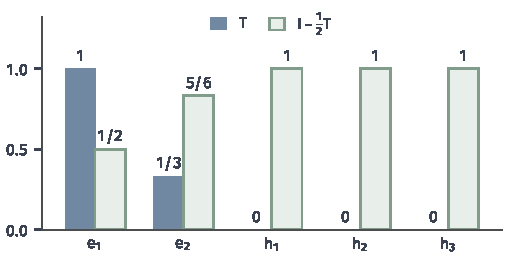
\includegraphics[width=86mm]{figures/04-spaces-measures-and-geometry/03-function-spaces/matplotlib/opeq-equation-types/figure.pdf}
  \caption{核$1+xz$（测度$\mathrm dz/2$）给出的两类方程在各正交方向上的乘子。$e_1=1$、$e_2=\sqrt3x$是特征方向，$h_1,h_2,h_3$代表与它们正交的方向（如$x^2-\frac13$）。蓝色为第一类方程的算子$T$，在正交方向上为零；绿色为第二类方程的算子$I-\frac12T$，在正交方向上恒为$1$。}
  \label{fig:opeq-equation-types}
\end{BookInlineFigure}

困难只出现在两个特殊参数上：$\lambda=1$时齐次方程$(I-T)u=0$有非零解$u=1$，$\lambda=3$时有非零解$u=x$。它们正是特征值$1$与$\frac13$的倒数。

两类方程可以使用同一个积分核，可解性却由整个算子的结构决定。第一类方程的困难来自$K$本身：零空间造成不唯一，像不够大造成无解。第二类方程只在$1/\lambda$恰为$K$的特征值时出问题。下面两个小节分别处理“$\lambda$足够小”与“$\lambda$任意”两种情形。

\subsection{Neumann级数}
\label{sec:opeq-neumann}

标量方程$(1-q)x=f$在$\lvert q\rvert<1$时有解$x=\sum_{n\geq0}q^nf$。算子方程可以照此办理，只要几何级数在算子范数下收敛。第~\ref{chap:operator-spectra}章已经用这个级数确定谱的位置；这里把它当作解方程的方法，需要的是截断之后的余项。

\begin{theorem}[Neumann级数]
\label{thm:opeq-neumann}
设$X$为Banach空间，$S\in\mathcal B(X)$且$\lVert S\rVert<1$。则$I-S$有定义在整个$X$上的有界逆，
\begin{equation}
  (I-S)^{-1}=\sum_{n=0}^{\infty}S^n,\qquad
  \lVert(I-S)^{-1}\rVert\leq\frac{1}{1-\lVert S\rVert},
  \label{eq:opeq-neumann}
\end{equation}
级数按算子范数收敛。并且部分和$P_N=\sum_{n=0}^NS^n$满足
\begin{equation}
  \bigl\lVert(I-S)^{-1}-P_N\bigr\rVert\leq\frac{\lVert S\rVert^{N+1}}{1-\lVert S\rVert}.
  \label{eq:opeq-neumann-remainder}
\end{equation}
\end{theorem}

\begin{proof}
由$\lVert S^n\rVert\leq\lVert S\rVert^n$，对$M>N$有
\[
  \lVert P_M-P_N\rVert\leq\sum_{n=N+1}^M\lVert S\rVert^n.
\]
右端是收敛几何级数的尾部，所以$(P_N)$在$\mathcal B(X)$中是Cauchy列。第~\ref{chap:linear-operators}章说明$X$完备时$\mathcal B(X)$完备，所以$P_N$收敛到某个$P$，并且
\[
  \lVert P\rVert\leq\sum_{n\geq0}\lVert S\rVert^n=\frac1{1-\lVert S\rVert}.
\]

逐项相乘时中间各项相消，部分和满足
\[
  P_N(I-S)=(I-S)P_N=I-S^{N+1}.
\]
由$\lVert S^{N+1}\rVert\leq\lVert S\rVert^{N+1}\to0$，令$N\to\infty$，得到$P(I-S)=(I-S)P=I$，所以$P$是$I-S$的有界逆。

最后，$P-P_N=\sum_{n>N}S^n$，逐项取范数并对几何级数求和，即得式~\eqref{eq:opeq-neumann-remainder}。
\end{proof}

级数$\sum_{n\geq0}S^n$称为\term{Neumann级数}（Neumann series）。取$S=\lambda K$，条件$\lVert S\rVert<1$就是$\lvert\lambda\rvert\lVert K\rVert<1$。此时第二类方程~\eqref{eq:opeq-second-kind}对每个$f$有唯一解
\begin{equation}
  u=\sum_{n=0}^\infty\lambda^nK^nf,\qquad
  \lVert u\rVert\leq\frac{\lVert f\rVert}{1-\lvert\lambda\rvert\lVert K\rVert}.
  \label{eq:opeq-neumann-solution}
\end{equation}
这一构造只用到小范数和空间的完备性，没有用到$K$的紧性。

\paragraph{截断与迭代}
实际计算只能保留有限项。记$q=\lvert\lambda\rvert\lVert K\rVert<1$，$u_N=\sum_{n=0}^{N}(\lambda K)^nf$。由式~\eqref{eq:opeq-neumann-remainder}，误差满足
\begin{equation}
  \lVert u-u_N\rVert\leq\frac{q^{N+1}}{1-q}\lVert f\rVert.
  \label{eq:opeq-neumann-truncation}
\end{equation}
误差按几何速度下降，$q$接近$1$时，同样的精度需要多得多的项。

部分和不必逐项计算$K^n$，可以递推：
\begin{equation}
  u_N=f+\lambda Ku_{N-1},\qquad u_{-1}=0.
  \label{eq:opeq-neumann-iteration}
\end{equation}
这就是不动点迭代$u\mapsto f+\lambda Ku$，也就是\BookChapterRef{chap:stationary-iterations}{卷二第11章“定常迭代法”}中步长取$1$的Richardson迭代的算子形式。这个映射满足
\[
  \lVert(f+\lambda Ku)-(f+\lambda Kw)\rVert\leq q\lVert u-w\rVert,
\]
是完备空间上的压缩映射，第~\ref{chap:metric-space-maps}章的压缩映射原理说明，从任意初值出发迭代都收敛到同一个解。

下面在秩二例子上走一遍，数据是
\[
  \lambda=\frac12,\qquad f=1+x.
\]
这时$\lVert T\rVert=1$，$q=\frac12$，由式~\eqref{eq:opeq-rank-two-second}，精确解为$u=2+\frac65x$。迭代的第一步是
\[
  u_0=1+x,\qquad
  u_1=f+\frac12Tu_0=\frac32+\frac76x.
\]

写$u_N=a_N+b_Nx$，式~\eqref{eq:opeq-neumann-iteration}给出两个系数各自的递推：
\[
  a_N=1+\frac12a_{N-1},\qquad b_N=1+\frac16b_{N-1}.
\]
解这两个递推，得到
\[
  a_N=2\bigl(1-2^{-(N+1)}\bigr),\qquad
  b_N=\frac65\bigl(1-6^{-(N+1)}\bigr).
\]
以$N=2$为例，$a_2=\frac74$，$b_2=\frac{43}{36}$。

一次多项式的范数由下式计算：
\[
  \lVert\alpha+\beta x\rVert^2=\lvert\alpha\rvert^2+\frac{\lvert\beta\rvert^2}3.
\]
代入系数的误差$\frac14$与$\frac1{180}$，$N=2$时的实际误差为
\[
  \sqrt{\Bigl(\frac14\Bigr)^2+\frac13\Bigl(\frac1{180}\Bigr)^2}\approx0.2500.
\]
由$\lVert f\rVert^2=\frac43$，式~\eqref{eq:opeq-neumann-truncation}给出的上界是$2^{-2}\cdot2/\sqrt3\approx0.2887$，只比实际误差大约$15\%$。

图~\ref{fig:opeq-neumann-convergence}显示，常数方向以$\frac12$的比率收敛，线性方向以$\frac16$的比率收敛；总误差由最慢的方向决定，这就是上界中$q$取算子范数的原因。

\begin{BookInlineFigure}
  \centering
  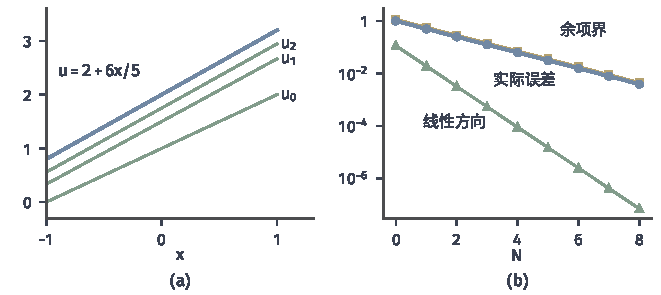
\includegraphics[width=112mm]{figures/04-spaces-measures-and-geometry/03-function-spaces/matplotlib/opeq-neumann-convergence/figure.pdf}
  \caption{$(I-\frac12T)u=1+x$的Neumann迭代。(a)绿色直线是迭代值$u_0,u_1,u_2$，蓝色直线是精确解。(b)对数纵轴上的误差：蓝色为实际误差，黄色为式~\eqref{eq:opeq-neumann-truncation}的上界，两者几乎平行；绿色为线性方向的误差，以$\frac16$的比率衰减，快于主导的常数方向。}
  \label{fig:opeq-neumann-convergence}
\end{BookInlineFigure}

\paragraph{小范数只是充分条件}
$\lvert\lambda\rvert\lVert K\rVert<1$保证可解，但远不是可解的必要条件。在秩二例子中取$\lambda=2$，常数方向的迭代系数满足$a_N=a+2a_{N-1}$，只要$a\neq0$就发散。可是$\lambda\neq1,3$，由式~\eqref{eq:opeq-rank-two-second}，方程对每个$f$仍有唯一解：
\[
  u=-a+3bx+r.
\]
取$f=1+x$，解为$u=-1+3x$。代回核对：$Tu=-1+x$，所以$u-2Tu=1+x$。方程可解与某种展开收敛是两件事。

反方向的例子是累积积分。$\lVert V\rVert=\sigma_1=2/\pi$，$\lambda=10$时$\lvert\lambda\rvert\lVert V\rVert>1$，定理的条件不成立，级数却仍然收敛。反复积分的公式是
\[
  (V^nf)(x)=\int_0^x\frac{(x-t)^{n-1}}{(n-1)!}f(t)\,\mathrm dt.
\]
由Cauchy--Schwarz不等式，$\lVert V^n\rVert\leq1/(n-1)!$，分母的增长压过任何$\lvert\lambda\rvert^n$。

所以$(I-\lambda V)u=f$对每个$\lambda$都有唯一解。取$f=1$，由$V^n1=x^n/n!$，得到
\[
  u(x)=\sum_{n=0}^\infty\frac{(\lambda x)^n}{n!}=e^{\lambda x}.
\]
$\lambda=10$时代回核对：$10Vu=e^{10x}-1$，所以$u-10Vu=1$。这与第~\ref{chap:operator-spectra}章的结论相符：$V$的谱只有$\{0\}$，没有非零特征值。要对所有参数判断可解性，需要用到$K$的紧性，这就是下一小节的内容。

\subsection{Fredholm可解条件}
\label{sec:opeq-fredholm}

先把参数分成情形。$\lambda=0$时方程就是$u=f$，总有唯一解。$\lambda\neq0$时，
\[
  I-\lambda K=-\lambda\Bigl(K-\frac1\lambda I\Bigr),
\]
所以齐次方程$(I-\lambda K)u=0$有非零解，当且仅当$1/\lambda$是$K$的特征值。

方阵有一个熟悉的事实：$\bm B\bm x=\bm 0$只有零解，当且仅当$\bm B\bm x=\bm b$对每个右端有解；若有非零解，则$\bm b$必须与$\bm B^\top$的零空间正交。下面说明，对$B=I-\lambda K$这个结论原样成立。先在紧自伴情形用特征方向看清答案，再对一般紧算子给出证明。

\paragraph{紧自伴情形的方向解释}
设$K$为紧自伴算子。为避免与参数$\lambda$混淆，记它的非零特征值为$\mu_j$。由第~\ref{chap:operator-spectra}章的谱分解，存在实数$\mu_j\neq0$与标准正交特征向量$e_j$，使每个$w\in H$写成$w=w_0+\sum_j\langle e_j,w\rangle e_j$，其中$w_0\in\ker K$；若特征值有无穷多个，则$\mu_j\to0$。把$I-\lambda K$作用在$u$上，得到
\[
  (I-\lambda K)u=u_0+\sum_j(1-\lambda\mu_j)\langle e_j,u\rangle e_j.
\]
$I-\lambda K$在零空间上是恒等作用，在第$j$个特征方向上乘以$1-\lambda\mu_j$。

若$\lambda$不等于任何$1/\mu_j$，这些乘子都不为零。又因为$\mu_j\to0$，乘子趋于$1$，只有有限个乘子离$1$较远，所以$\inf_j\lvert1-\lambda\mu_j\rvert>0$。逐方向除以乘子就得到有界逆：
\begin{equation}
  u=f_0+\sum_j\frac{\langle e_j,f\rangle}{1-\lambda\mu_j}e_j,
  \label{eq:opeq-self-adjoint-solution}
\end{equation}
其中$f_0$是$f$在$\ker K$上的分量。

若$\lambda=1/\mu_k$，乘子在$\mu_k$的特征空间上为零。这个特征空间有限维，就是齐次方程的解空间。此时方程可解，当且仅当$f$在这些方向上的系数为零，即$f\perp\ker(I-\lambda K)$；解可以加上该特征空间中的任意元素。

秩二例子中，$\lambda=1$时方程$(I-T)u=f$可解当且仅当$a=\langle1,f\rangle=0$。此时由式~\eqref{eq:opeq-rank-two-second}，第二个方程给出$\frac23\beta=b$，解为
\[
  u=c+\frac32bx+r,\qquad c\text{任意}.
\]
图~\ref{fig:opeq-fredholm-alternative}(a)画出三个乘子随$\lambda$的变化。除$\lambda=1,3$这两个参数外方程总是唯一可解，$\lambda=\frac12$与$\lambda=2$都在这个范围内，虽然只有前者满足小范数条件。

\begin{BookInlineFigure}
  \centering
  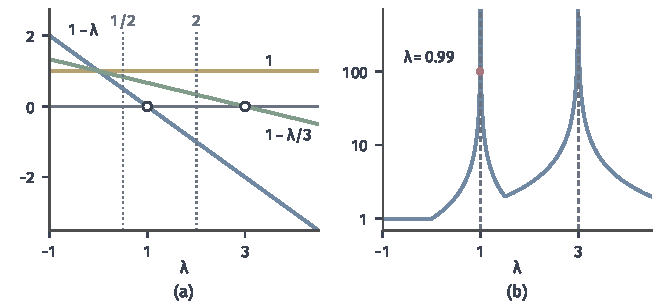
\includegraphics[width=112mm]{figures/04-spaces-measures-and-geometry/03-function-spaces/matplotlib/opeq-fredholm-alternative/figure.pdf}
  \caption{第二类方程$(I-\lambda T)u=f$对参数的依赖（核$1+xz$，测度$\mathrm dz/2$）。(a)三个方向的乘子：蓝色$1-\lambda$、绿色$1-\lambda/3$、黄色恒为$1$。空心圆处乘子为零，是例外参数；点线标出$\lambda=\frac12$（满足小范数条件）与$\lambda=2$（不满足，但仍唯一可解）。(b)逆算子的范数，对数纵轴，在两个例外参数处趋于无穷；红点为$\lambda=0.99$，范数$100$。}
  \label{fig:opeq-fredholm-alternative}
\end{BookInlineFigure}

\paragraph{Fredholm择一}
一般紧算子没有正交特征基可用，但结论的形式保持不变，只是正交条件要改用伴随方程的零空间。

\begin{theorem}[Fredholm择一]
\label{thm:opeq-fredholm}
设$H$为Hilbert空间，$K:H\to H$为紧算子，$\lambda\in\mathbb F$，$B=I-\lambda K$。则
\begin{enumerate}
  \item $\ker B$与$\ker B^*$都是有限维的，且$\dim\ker B=\dim\ker B^*$；
  \item $\operatorname{Ran}B$是闭子空间，因而$\operatorname{Ran}B=(\ker B^*)^\perp$；
  \item $\ker B=\{0\}$当且仅当$\operatorname{Ran}B=H$，此时$B^{-1}$有界。
\end{enumerate}
因此以下两种情形恰有一种成立。或者齐次方程$Bu=0$只有零解，此时对每个$f\in H$，方程$Bu=f$有唯一解，解由有界算子$B^{-1}$给出。或者齐次方程有非零解，此时$Bu=f$可解当且仅当$f\perp\ker B^*$，全部解为一个特解加上有限维子空间$\ker B$中的任意元素。
\end{theorem}

这一结论称为\term{Fredholm择一}（Fredholm alternative）。其中$B^*=I-\overline\lambda K^*$。取伴随方程$B^*w=0$的解空间的一组基$w_1,\ldots,w_r$，可解条件就是有限个等式
\begin{equation}
  \langle w_i,f\rangle=0,\qquad i=1,\ldots,r,
  \label{eq:opeq-compatibility}
\end{equation}
称为方程的\term{相容条件}（compatibility condition）。非唯一来自有限维的$\ker B$，不可解来自数据违反有限个相容条件，满足这些条件的数据都可解。

定理的关键是第二条。像的闭性由紧性事先保证，所以正交条件$f\perp\ker B^*$判断的是精确可解，而不只是$f$能否被输出逼近。上一节的对角算子$A$正好相反：每个数据都满足正交条件，但$A$的像不闭，$(1/n)$不在其中。

为什么条件要看伴随的零空间，而不是$\ker B$本身？用一个不自伴的例子说明。在$L^2(0,1)$上取秩一算子
\[
  (Ku)(x)=x\int_0^1u(z)\,\mathrm dz,
\]
并取$\lambda=2$，$B=I-2K$。

直接计算两个零空间。$u=x$满足$Ku=\frac12x$，所以$\ker B=\operatorname{span}\{x\}$。伴随是$(K^*w)(z)=\int_0^1xw(x)\,\mathrm dx$，输出总是常函数，代入$w=1$得$K^*1=\frac12$，所以$\ker B^*=\operatorname{span}\{1\}$。

把方程$u-2x\int_0^1u=f$两边在$[0,1]$上积分，左边是$\int u-2\cdot\frac12\int u=0$，所以
\[
  \int_0^1f(x)\,\mathrm dx=0
\]
是必要条件，这正是$f\perp1$，不是$f\perp x$。例如$f=2x-1$满足这个条件，全部解为$u=2x-1+cx$，而它与$x$并不正交，$\langle x,f\rangle=\frac16$。$f=1$违反条件，方程无解。

\paragraph{有限秩部分与小范数余项}
证明的想法是把紧算子拆成两部分：有限秩部分化成有限维线性方程组，余项用Neumann级数吸收。这样，无限维方程的可解性就完全由一个方阵决定。$\lambda=0$时$B=I$，结论直接成立，下面设$\lambda\neq0$。

\begin{proof}
第一步，分解。由第~\ref{chap:linear-operators}章，Hilbert空间上的紧算子能按算子范数被有限秩算子逼近。取有限秩算子$F$使$\lVert\lambda(K-F)\rVert<1$，记$C=I-\lambda(K-F)$。由定理~\ref{thm:opeq-neumann}，$C$有有界逆，于是
\[
  B=C-\lambda F=C(I-G),\qquad G=\lambda C^{-1}F.
\]

$G$仍是有限秩的有界算子。取$\operatorname{Ran}G$的一组基$b_1,\ldots,b_r$，则$Gu=\sum_{i=1}^r\ell_i(u)b_i$。系数$\ell_i$是有界线性泛函，因为有限维空间上的坐标泛函连续，与有界的$G$复合仍有界。由Riesz表示写成$\ell_i(u)=\langle a_i,u\rangle$，于是
\[
  Gu=\sum_{i=1}^r\langle a_i,u\rangle b_i.
\]

第二步，化为矩阵方程。令$\bm M$是$r\times r$矩阵，$\bm M_{i,j}=\langle a_i,b_j\rangle$，并记
\[
  \bm d(h)=(\langle a_1,h\rangle,\ldots,\langle a_r,h\rangle)^\top.
\]
我们断言：$(I-G)u=h$当且仅当$u=h+\sum_ic_ib_i$，其中$\bm c$满足
\[
  (\bm I-\bm M)\bm c=\bm d(h).
\]

若$(I-G)u=h$，则$u=h+Gu=h+\sum_ic_ib_i$，其中$c_i=\langle a_i,u\rangle$。把$u$的表达式代入这个内积，得到
\[
  c_i=\langle a_i,h\rangle+\sum_j\bm M_{i,j}c_j.
\]
反过来，若$\bm c$满足矩阵方程，令$u=h+\sum_jc_jb_j$，则
\[
  \langle a_i,u\rangle=\bm d(h)_i+(\bm M\bm c)_i=c_i,
\]
所以$Gu=\sum_ic_ib_i=u-h$。

第三步，像是闭的。由第二步，$h\in\operatorname{Ran}(I-G)$当且仅当$\bm d(h)\in\operatorname{Ran}(\bm I-\bm M)$。有限维子空间$\operatorname{Ran}(\bm I-\bm M)$是闭集，$\bm d$连续，所以$\operatorname{Ran}(I-G)$作为闭集的原像是闭的。$C$及其逆都连续，把闭集映成闭集，所以
\[
  \operatorname{Ran}B=C\bigl(\operatorname{Ran}(I-G)\bigr)
\]
闭。再由第~\ref{chap:linear-operators}章的关系$\overline{\operatorname{Ran}B}=(\ker B^*)^\perp$，第二条结论成立。

第四步，比较两个零空间的维数。取$h=0$，第二步说明$\bm c\mapsto\sum_ic_ib_i$是$\ker(\bm I-\bm M)$到$\ker(I-G)$的线性双射，这里用到$b_i$线性无关。$C$可逆，所以$\ker B=\ker(I-G)$，于是
\[
  \dim\ker B=\dim\ker(\bm I-\bm M).
\]

伴随一侧同样计算。由内积的共轭线性，$G^*w=\sum_i\langle b_i,w\rangle a_i$。若$w=G^*w$，令$d_i=\langle b_i,w\rangle$，则$w=\sum_jd_ja_j$，再与$b_i$作内积，得到
\[
  d_i=\sum_j\langle b_i,a_j\rangle d_j,
\]
这正是$\bm d=\bm M^{\mathsf H}\bm d$。反过来，每个满足此式的$\bm d$都给出$w=\sum_jd_ja_j\in\ker(I-G^*)$，且$w$确定$\bm d$，所以两个解空间线性同构。

又$B^*=(I-G^*)C^*$，$C^*$可逆，所以$\ker B^*$与$\ker(I-G^*)$维数相同。方阵与其共轭转置的秩相等，于是
\[
  \dim\ker B^*=\dim\ker(\bm I-\bm M^{\mathsf H})=\dim\ker(\bm I-\bm M)=\dim\ker B.
\]
这个公共的维数不超过$r$，第一条结论成立。

第五步，单射与满射等价。若$\ker B=\{0\}$，由第四步$\ker B^*=\{0\}$，再由第二条，$\operatorname{Ran}B=H$。反之，若$\operatorname{Ran}B=H$，则$\ker B^*=(\operatorname{Ran}B)^\perp=\{0\}$，由第四步$\ker B=\{0\}$。双射的有界算子$B$的逆有界，这由第~\ref{chap:linear-operators}章的开映射定理保证。
\end{proof}

用前面的秩一算子走一遍证明。这里$K$已是有限秩，取$F=K$，则$C=I$，$G=\lambda K$，只需一个基$b_1=x$，$a_1=\lambda\cdot1$（取实数$\lambda$），于是
\[
  \bm M=\langle a_1,b_1\rangle=\frac\lambda2,\qquad \bm d(h)=\lambda\int_0^1h.
\]
矩阵方程是一个标量方程：
\[
  \Bigl(1-\frac\lambda2\Bigr)c=\lambda\int_0^1h(x)\,\mathrm dx.
\]

$\lambda=1$时，$c=2\int h$，解为$u=h+2x\int_0^1h$。取$h=1$得$u=1+2x$，代回核对：$\int_0^1u=2$，所以$u-x\int_0^1u=1$。$\lambda=2$时，标量方程变成$0\cdot c=2\int h$，要求$\int h=0$，且$c$任意，这正是前面得到的相容条件和解的结构。

无限维方程的全部可解性就这样落在一个矩阵上，无限维的部分被可逆的$C$吸收了。这也说明了紧性的作用：若$K$不能被有限秩算子逼近，就无法这样把问题化到有限维。另一方面，定理只说明解存在并有界地依赖于数据，并不给出收敛的迭代格式，前面$\lambda=2$的例子正处于“唯一可解但Neumann级数发散”的情形。

定理的第三条也与第~\ref{chap:operator-spectra}章的结论一致：若$\mu\neq0$不是紧算子$K$的特征值，取$\lambda=1/\mu$，则$I-\lambda K$是单射，因而有有界逆，$K-\mu I=-\mu(I-\lambda K)$也有有界逆。所以紧算子的非零谱点都是特征值。这里的证明只用到有限秩逼近和Neumann级数，是这一事实的另一条论证路线。
